\chapter{Brief History: Farming} \label{g:history}
The history of humans can be explained in a quest to be calorie efficient \cite{stephenfry2018}. Calorie is a unit for energy, and energy is the only universal currency \cite{energy2017VaclavSmil}. Early people understood this and began altering their land, and its flora and fauna, in the quest for energy efficiency. When our ancestors went from foraging to farming, we went from mobility to sedentism, which is more energy efficient. 

Two laws will always govern our quest for energy efficiency: (1) energy can be changed from one form to another without any loss of total energy (the 1\textsuperscript{st} law of thermodynamics); and (2) in its conversion there is always an inevitable loss of useful energy to a gain in entropy (2\textsuperscript{nd} law of thermodynamics). Farmers have used tools, human, animal, and mental labor, to maximize the change of one form of energy into another while minimizing the loss of useful energy to entropy or heat. In doing so, farmers attempt to efficiently change the sun's heat energy to food calories, or the work of muscle to potential energies when harvesting and processing plants. In every step, they try to maximize the change of energy types while minimizing losses of energy. For example, using a sickle maximizes the work of the arm yielding it, and using a sharp sickle minimizes the frictional losses. Most farming work today happens in the form of mental labor and even though mental labor is still labor, in terms of energy expenditures, it falls short of muscle work.

Looking at farming through the energy lens explains why both constancy and change mark its history. Once an agricultural system reaches the maximum efficiency possible under the current order, people can decide to stay and stabilize their population, to let their numbers decline, to migrate, or to adopt a more productive way of farming. In other words, they can chose constancy or change, while change almost definitely requires a higher energy input \cite{energy2017VaclavSmil}. This concept is analogous to the \textit{activation energy} some chemical reactions require. With a large enough activation energy, we can upset the equilibrium state and push the current order to a new state. In essence, the energy requirements or activation energy ``hill" deters change, when change is required and desired for growth. 
 
%\begin{enumerate}
%	\item The use of simple tools (e.g., the sickle and the plow) to make human labor more efficient, and the evolution of these tools
%	\item The partial outsourcing of human labor to animals
%	\item The harvesting of renewable sources of energy (i.e., water and wind) for grain processing (e.g, milling and oil extraction)
%	\item The control over irrigation and fertilizer, which removed the two key constraints (i.e., water and nitrogen) on crop yields \cite{energy2017VaclavSmil}
%	\item The shift to more intensive systems of land use (multicropping or in rotation), under the pressure of increasing population, leading to resiliency and higher yields \cite{sovani1966boserup}
%	\item More advancements in tools (e.g., from the 1800s to the 1900s, harvesting equipment went from sickle to cradle, binder, then combine; the plow went from wooden to cast-iron, steel, then steel gang) all increasing efficiency in human labor
%	\item The production of fertilizers (i.e., nitrogen, phosphorus, and potassium, and later the production of synthetic nitrogenous fertilizers). 
%	\item The use of pesticides to control disease
%	\item The use of non-renewable sources of energy (i.e., fossil fuels) for operating machines like tractors and trucks \cite{energy2017VaclavSmil}.  
%	\item Labor turning to supporting, controlling, and managing the productive process
%	\item The harvesting of another renewable source of energy (i.e., solar)
%	\item The mental development of expertise, which also requires energy inputs
%	\item The collection of data and the outsourcing of our expertise, and more to the point, our decision making, to machines
%\end{enumerate}

\begin{figure}[ht]
	\centering
	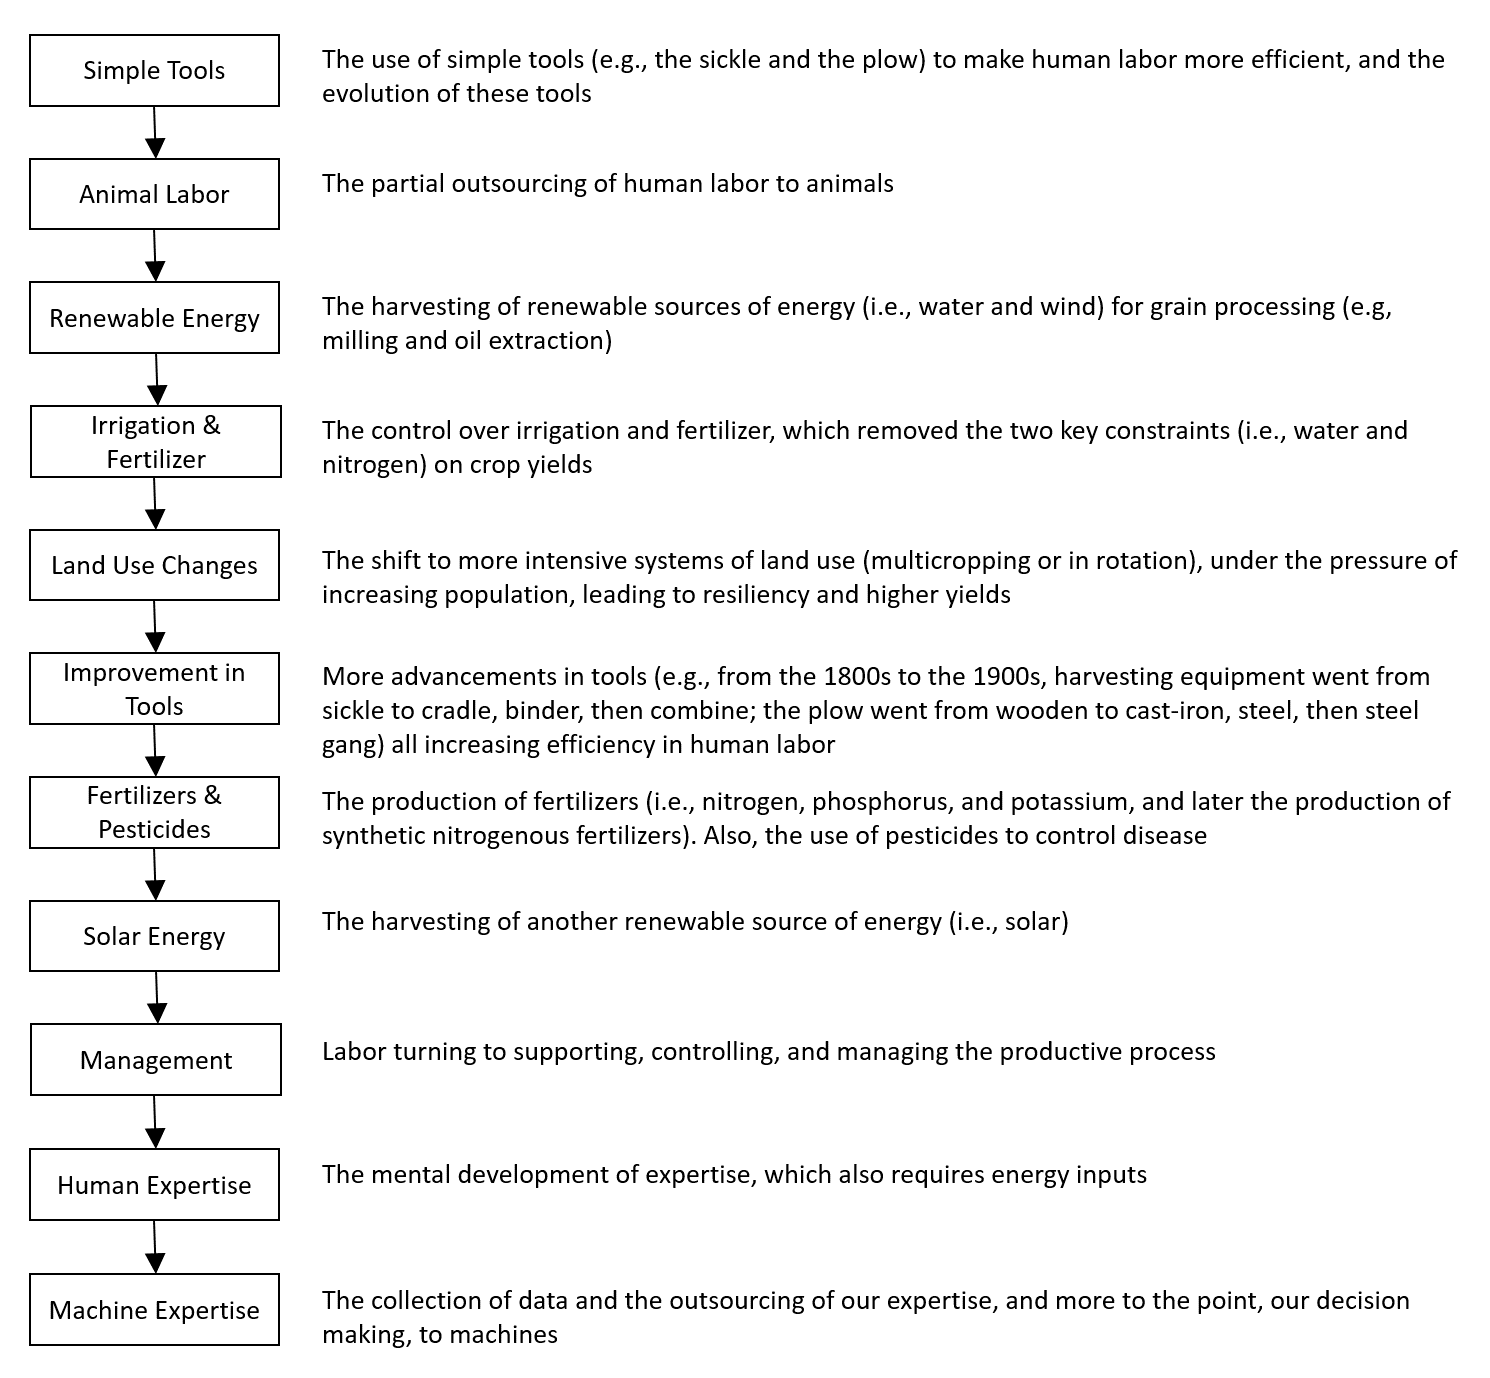
\includegraphics[width=\textwidth,trim={0 0 0 0},clip=true]{Plots/farmingsteps.png}
	\caption{Change, growth, and, eventually, higher yields in farming have come from these developments throughout history.} 
	\label{fig:farmingsteps}
\end{figure}

From the first development in farming in Figure \ref{fig:farmingsteps} to the most recent advances in statistical learning, the changes outlined above have occurred to remove all the removable limits to production. That is, with each expenditure of activation energy we were able to remove another limit to growth. Each time arriving at another limit. Today, we have yet to completely optimizing our farming practices, engineer our weather systems, and to completely replace human labor. As it was customary for farming families to have a lot of children, machine learning and artificial intelligence may be our era's way of outsourcing our species mental labor, until, ultimately, we replace our own agency with the programmed agenda. This ultimate goal, and our recent wage stagnation, a jobless economic recovery, and rapid improvements in Big Data and artificial intelligence have again stoked the fear of mass unemployment that has always haunted labor-saving technology \cite{frase2016four}. 








